\newpage
\section{Appraisal}
\subsection{System Appraisal}
Multiple methods were used to ascertain the completeness of the application these will be discussed in 
relevance to the ends of the system.
\subsubsection{Back-end}
The back-end of the system was appraised partly through user testing as will be discussed in the 
front-end section next. But primarily through the use of unit and integration tests using jest \cite{jest}.
Testing was brought to 99\%+ coverage in all source files as shown by the overall report in Figure \RefFig{fig:coverage} and 
shown in Appendix V.
\begin{figure}[h]
    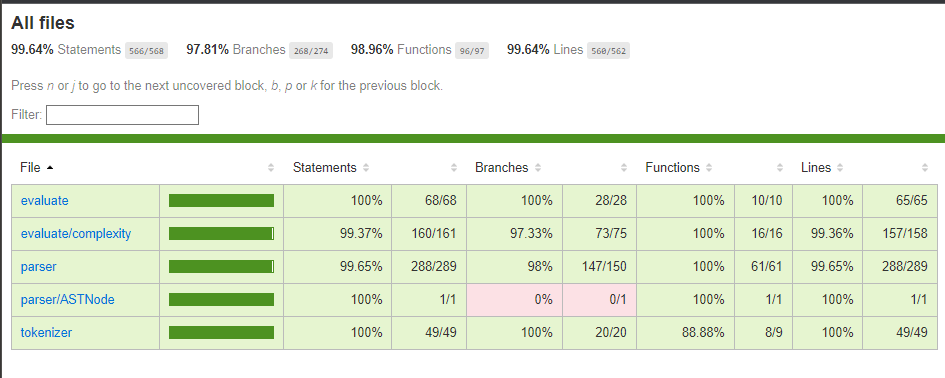
\includegraphics[width=.5\textwidth]{images/coverage.png}
    \caption{Testing Coverage See Appendix V}
    \Description{Testing Coverage  See Appendix V}
    \label{fig:coverage}
\end{figure}

\subsubsection{Front-end}
The front end of the system was tested via user evaluation.
\newline
The first of these was a questionnaire on the code editor \cite{codeeditortesting} which was accompanied with the 
participant information sheet and informed consent information. The questionnaire asked the users to voice their opinion qualitatively 
on the artifact. The responses were mixed, most liked the dark design of the application, although there were comments 
that the code editor was too simple and needed more features, this is what prompted the implementation of the autocomplete and autofill 
features.
\begin{figure}[h]
    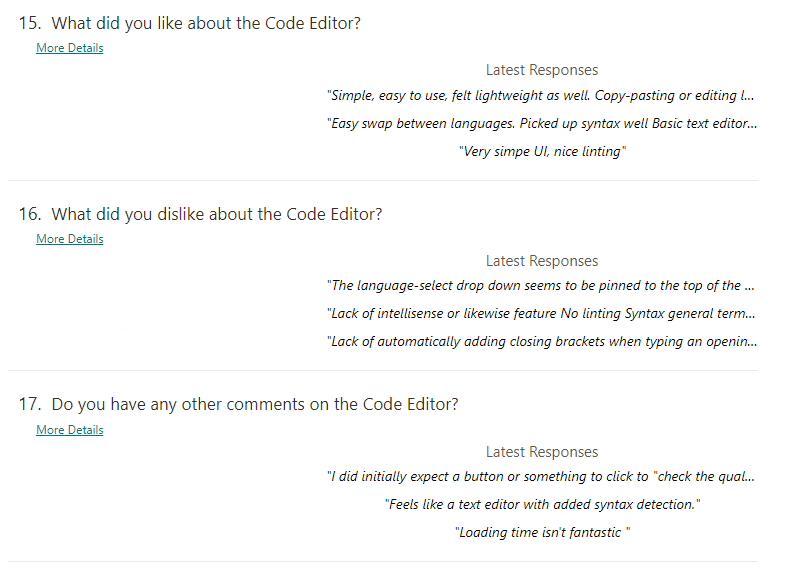
\includegraphics[width=.5\textwidth]{images/responses-code-editor.png}
    \caption{Responses to the code editor testing}
    \Description{Responses to the code editor testing}
    \label{fig:responses}
\end{figure}
\newline
Another deployment was created with the updated features \cite{codeeditortesting2}.
The previous questionnaire prompted users to email the student if they wanted to participate in more testing, there was a 
response and an interview conducted. The user was asked to further use the system as they normally would and to use the 
new autocomplete and autofill features. The user commented that they liked the new features and especially like that 
it autofilled words they had previously entered. This session also unearthed a bug where in large files autocomplete would stop working 
which was fixed. They also mentioned that they wanted to be able to click to autocomplete, this feature did not end up being implemented.
See Appendix W for anonymised interview notes.
\newline
\newline
Finally the system was evaluated by the use of a Questionnaire. The final system was deployed \cite{finalTesting} and users were prompted to evaluate the system quantitatively.
As shown in Figure \RefFig{fig:responses2} users were happy with the analysis output panels with 100\% of responses being Agree or Strongly Agree. 
Sentiment towards the code editor was mixed but remained neutral at worst. 67\% of responses strongly agreed that this application had made them more interested in 
code quality analysis, this is 
\begin{figure}[h]
    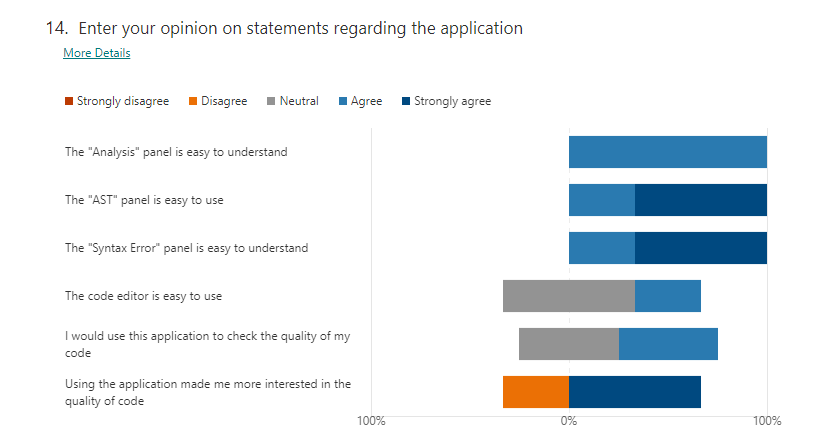
\includegraphics[width=.5\textwidth]{images/finaltestingopinion.png}
    \caption{Responses to the final testing}
    \Description{Responses to the final testing}
    \label{fig:responses2}
\end{figure}

\subsection{Appraisal of Work}
I believe that work was generally good on the project. If I was to do this project again I would likely use 
a pre-made parser, this would have made the project so much easier and allowed for more to be accomplished during the project, understanding this 
it was a learning experience that has given the student deeper understanding of how parsing works.
\newline
I would have also spent less time on research and more time on development, again this gave me a deep understanding of the subject matter but more time for 
development would have been beneficial.
